\section{高速化に対する粘度比の影響}
\label{sec:viscosity}
先行研究である岩室\cite{ref:8}において,超音波照射による高速化は,球の落下による粘度$\mu_\text{U}$と超音波照射による音響境界層内粘度$\mu_\text{ABL}$の比に,落下球の半径$a$で規格化された音響境界層内厚さ$\delta$を乗じた値で整理できると示された.この手法を用いて,\ref{sec:density},\ref{sec:concentration},\ref{sec:diameter}章に示した各実験結果を整理する.式(\ref{eq:Udiff})より,球の落下による粘度$\mu_\text{U}$と超音波照射による音響境界層内粘度$\mu_\text{ABL}$の比に,落下球の半径$a$で規格化された音響境界層内厚さ$\delta$を乗じた値と高速化度合いの関係をFig.\ref{fig:viscosity_ratio}に示す.

横軸が0.1までの範囲において,超音波照射による高速化度合いと粘度比と音響境界層を球の半径で規格化した値は,正の相関関係にある.しかし,0.1を越えるとばらつきが大きくなり,まったく高速化が見られない条件も存在した.その後,横軸が増加していくと0.1以下より緩やかに高速化が現れるようになった.これより,超音波照射による高速化に関して,横軸の値が0.1より小さい値では正の相関がみられるが,それ以上では粘度,音響境界層厚さ,落下球の半径以外の要因で超音波照射による高速化が抑制されていると考えられる.落下球の半径が小さい場合,擬塑性流体の粘度が大きい場合,落下球と流体の密度差が小さい場合,横軸の値が大きくなる.これらはすべて,擬塑性流体中を球が落下する際の終端速度が遅い場合である.この要因として,先行研究である岩室\cite{ref:8}において弾性による影響が示唆されている.本研究\ref{sec:elasticity-discussion}章にて,それらの議論を行う.

\begin{figure}[ht]
    \centering
    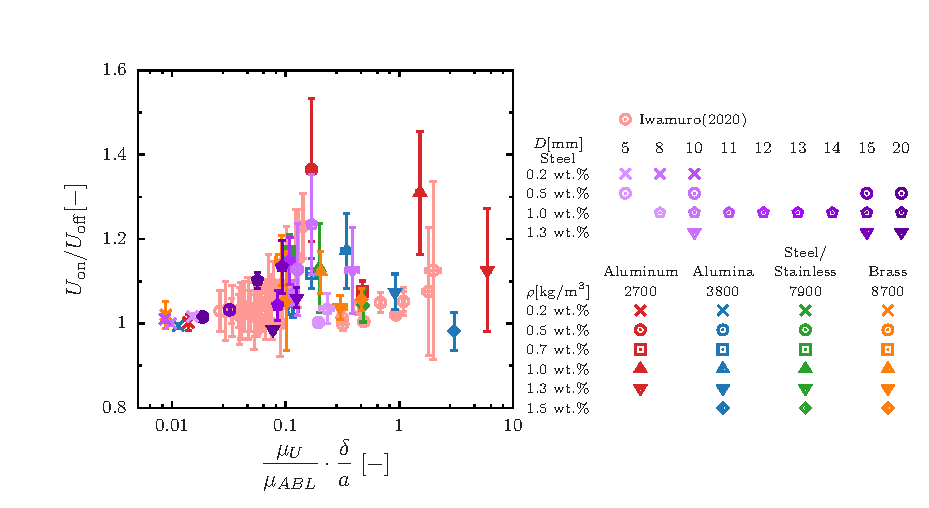
\includegraphics[width=1.0\textwidth]{5-Results/viscosity.eps}
    \caption{Relationship between velocity ratio and the inverse of the viscosity ratio multiplied by the thickness.}
    \label{fig:viscosity_ratio}
\end{figure}
